% Этот шаблон документа разработан в 2014 году
% Данилом Фёдоровых (danil@fedorovykh.ru) 
% для использования в курсе 
% <<Документы и презентации в \LaTeX>>, записанном НИУ ВШЭ
% для Coursera.org: http://coursera.org/course/latex .
% Исходная версия шаблона --- 
% https://www.writelatex.com/coursera/latex/5.1

\documentclass[c]{beamer}  % [t], [c], или [b] --- вертикальное выравнивание на слайдах (верх, центр, низ)
%\documentclass[handout]{beamer} % Раздаточный материал (на слайдах всё сразу)
%\documentclass[aspectratio=169]{beamer} % Соотношение сторон

% \usetheme{Berkeley} % Тема оформления
%\usetheme{Bergen}
%\usetheme{Szeged}
% \usetheme{Warsaw}
\usetheme{Copenhagen}

% \usecolortheme{beaver} % Цветовая схема
%\useinnertheme{circles}
%\useinnertheme{rectangles}

%%% Работа с русским языком
\usepackage{cmap}					% поиск в PDF
\usepackage{mathtext} 				% русские буквы в формулах
\usepackage[T2A]{fontenc}			% кодировка
\usepackage[utf8]{inputenc}			% кодировка исходного текста
\usepackage[english,russian]{babel}	% локализация и переносы

%% Beamer по-русски
\newtheorem{rtheorem}{Теорема}
\newtheorem{rproof}{Доказательство}
\newtheorem{rexample}{Пример}

%%% Дополнительная работа с математикой
\usepackage{amsmath,amsfonts,amssymb,amsthm,mathtools} % AMS
\usepackage{icomma} % "Умная" запятая: $0,2$ --- число, $0, 2$ --- перечисление

\usepackage{ragged2e} % Выравнивание

%% Номера формул
%\mathtoolsset{showonlyrefs=true} % Показывать номера только у тех формул, на которые есть \eqref{} в тексте.
%\usepackage{leqno} % Нумерация формул слева

%% Свои команды
\DeclareMathOperator{\sgn}{\mathop{sgn}}

%% Перенос знаков в формулах (по Львовскому)
\newcommand*{\hm}[1]{#1\nobreak\discretionary{}
{\hbox{$\mathsurround=0pt #1$}}{}}

%%% Работа с картинками
\usepackage{graphicx}  % Для вставки рисунков
\graphicspath{{images/}{images2/}}  % папки с картинками
\setlength\fboxsep{3pt} % Отступ рамки \fbox{} от рисунка
\setlength\fboxrule{1pt} % Толщина линий рамки \fbox{}
\usepackage{wrapfig} % Обтекание рисунков текстом

%%% Работа с таблицами
\usepackage{array,tabularx,tabulary,booktabs} % Дополнительная работа с таблицами
\usepackage{longtable}  % Длинные таблицы
\usepackage{multirow} % Слияние строк в таблице

%%% Программирование
\usepackage{etoolbox} % логические операторы

%%% Другие пакеты
\usepackage{lastpage} % Узнать, сколько всего страниц в документе.
\usepackage{soul} % Модификаторы начертания
\usepackage{csquotes} % Еще инструменты для ссылок
%\usepackage[style=authoryear,maxcitenames=2,backend=biber,sorting=nty]{biblatex}
\usepackage{multicol} % Несколько колонок

%%% Картинки
\usepackage{tikz} % Работа с графикой
\usepackage{pgfplots}
\usepackage{pgfplotstable}
\usepackage{hyperref}

% \input{definitions.tex}
\addto\captionsrussian{\renewcommand{\figurename}{Рисунок}}

\title[Решение задачи регрессии]{Решение задачи регрессии \\ с помощью методов машинного обучения}
% \subtitle{}
\author{Голиков М. О.}
\date{19 декабря 2020}
\institute[ОГУ им. И. С. Тургенева]{<<ОРЛОВСКИЙ ГОСУДАРСТВЕННЫЙ УНИВЕРСИТЕТ \\ ИМЕНИ И.\,С.\,ТУРГЕНЕВА>>}

\begin{document}
	\frame[plain]{\titlepage}	% Титульный слайд
  \begin{frame}
    \hypersetup{colorlinks=true,linkcolor=blue,urlcolor=blue}
		\frametitle{Содержание}
		\tableofcontents
  \end{frame}

	\section{Описание исходных данных}
	\begin{frame}
    \frametitle{\insertsection}

    В данной работе используются \textbf{\href{https://www.kaggle.com/mirichoi0218/insurance}{данные}} о
    страховых выплатах медицинскому персоналу.

    \begin{figure}[H]
			\centering
			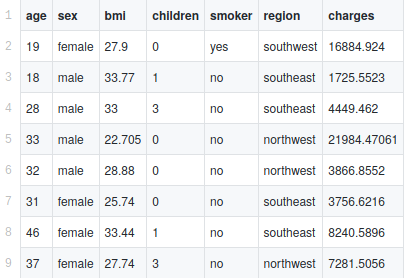
\includegraphics[scale=0.45]{data_example.png}
			\caption{Пример данных}
			\label{img:data_example}
		\end{figure}
	\end{frame}

	\begin{frame}
		\frametitle{\insertsection}

		Описание признаков:
		\begin{itemize}
			\item age - возраст бенефициара (лица, получающего страховые выплаты);
			\item sex - пол бенефициара;
			\item bmi - индексы массы тела;
			\item children - количество детей бенефициара, на которых распространяется страхование / количество иждевенцов бенефициара;
			\item smoker - является ли бенефициар курильщиком;
			\item region - жилой район бенефициара в США: северо-восток, юго-восток, юго-запад, северо-запад;
			\item charges - индивидуальные медицинские расходы, выставленные на счет медицинского страхования.
		\end{itemize}
	\end{frame}

	\section{Анализ данных}
	\begin{frame}
		\frametitle{\insertsection}

		\begin{block}{Гистограммы признаков sex и region}
			\begin{columns}[onlytextwidth,T]
				\column{0.5\textwidth}
				\begin{figure}[H]
					\centering
					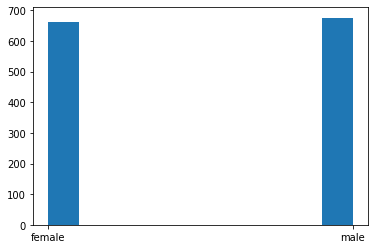
\includegraphics[scale=0.35]{sex_hist.png}
					\caption{Гистограмма признака sex}
					\label{img:sex_hist}
				\end{figure}
				\column{0.5\textwidth}
				\begin{figure}[H]
					\centering
					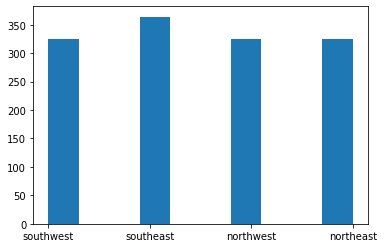
\includegraphics[scale=0.35]{region_hist.png}
					\caption{Гистограмма признака region}
					\label{img:region_hist}
				\end{figure}
			\end{columns}
		\end{block}
	\end{frame}

	\begin{frame}
		\frametitle{\insertsection}

		\begin{block}{Гистограммы признаков children и smoker}
			\begin{columns}[onlytextwidth,T]
				\column{0.5\textwidth}
				\begin{figure}[H]
					\centering
					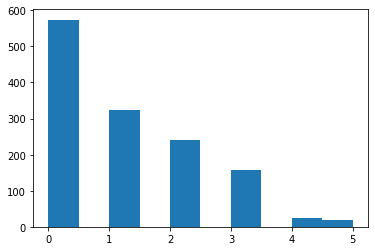
\includegraphics[scale=0.35]{children_hist.png}
					\caption{Гистограмма признака children}
					\label{img:children_hist}
				\end{figure}
				\column{0.5\textwidth}
				\begin{figure}[H]
					\centering
					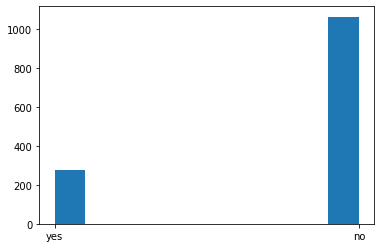
\includegraphics[scale=0.35]{smoker_hist.png}
					\caption{Гистограмма признака smoker}
					\label{img:smoker_hist}
				\end{figure}
			\end{columns}
		\end{block}
	\end{frame}

	\begin{frame}
		\frametitle{\insertsection}
		\justifying
		С помощью гистограмм удалось выяснить, что в категориальных признаках нет категорий, у которых
		была бы значительная количественная разница по отношению к другим значениям.
	\end{frame}

	\begin{frame}
		\frametitle{\insertsection}

		\begin{block}{Гистограммы признаков sex и region}
			\begin{columns}[onlytextwidth,T]
				\column{0.5\textwidth}
				\begin{figure}[H]
					\centering
					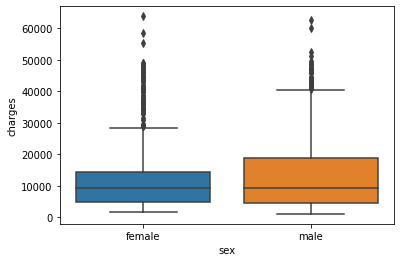
\includegraphics[scale=0.35]{sex_boxplot.png}
					\caption{Гистограмма признака sex}
					\label{img:sex_boxplot}
				\end{figure}
				\column{0.5\textwidth}
				\begin{figure}[H]
					\centering
					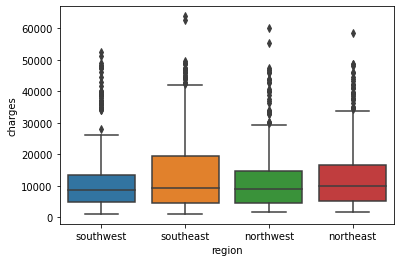
\includegraphics[scale=0.35]{region_boxplot.png}
					\caption{Гистограмма признака region}
					\label{img:region_boxplot}
				\end{figure}
			\end{columns}
		\end{block}
	\end{frame}

	\begin{frame}
		\frametitle{\insertsection}

		\begin{block}{Гистограммы признаков children и smoker}
			\begin{columns}[onlytextwidth,T]
				\column{0.5\textwidth}
				\begin{figure}[H]
					\centering
					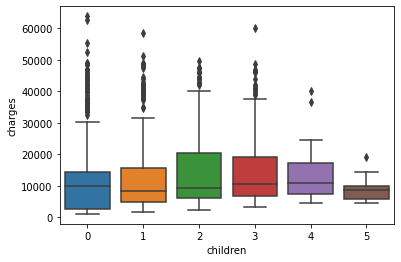
\includegraphics[scale=0.35]{children_boxplot.png}
					\caption{Гистограмма признака children}
					\label{img:children_boxplot}
				\end{figure}
				\column{0.5\textwidth}
				\begin{figure}[H]
					\centering
					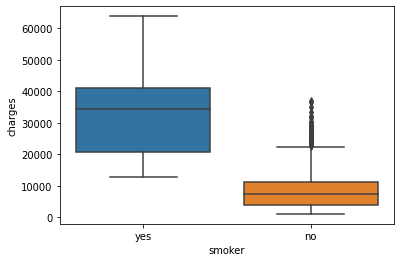
\includegraphics[scale=0.35]{smoker_boxplot.png}
					\caption{Гистограмма признака smoker}
					\label{img:smoker_boxplot}
				\end{figure}
			\end{columns}
		\end{block}
	\end{frame}

	\begin{frame}
		\frametitle{\insertsection}

		\begin{columns}[onlytextwidth,T]
			\column{0.5\textwidth}
			\justifying
			Справа можно увидеть диаграмму рассеяния и распределения признаков. Можно заметить, что между
			признаками не наблюдается линейной зависимости.
			
			Стоит обратить внимание на распределение признака charges, которое сильно
			скошено в левую сторону.
			\column{0.5\textwidth}
			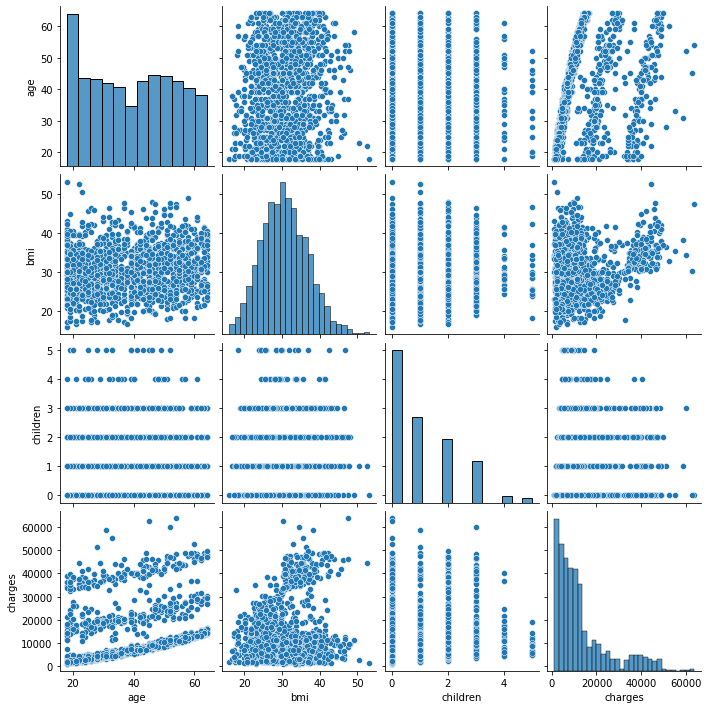
\includegraphics[scale=0.2]{scatterplot.png}
		\end{columns}
	\end{frame}

	\begin{frame}
		\frametitle{\insertsection}

		\begin{columns}[onlytextwidth,T]
			\column{0.7\textwidth}
			\justifying
			На рисунке справа представлена визуализация матрицы корреляции. На основе этих данных можно
			сделать вывод, что между вещественными признаками не наблюдается линейной зависимости, а также
			отсутсвует мультиколлинеарность.
			\column{0.3\textwidth}
			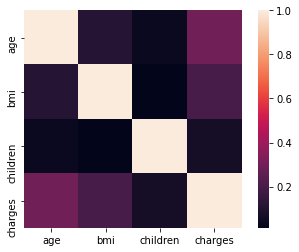
\includegraphics[scale=0.35]{correlation_matrix.png}
		\end{columns}
	\end{frame}

	\begin{frame}
		\frametitle{\null}

		Спасибо за внимание!
	\end{frame}
\end{document}
